\documentclass{standalone}
\usepackage{tikz}
\usepackage{ctex,siunitx,upgreek}
\setCJKmainfont{Noto Serif CJK SC}
\usepackage{tkz-euclide}
\usepackage{amsmath}
\usetikzlibrary{patterns, calc,3d}
\usetikzlibrary {decorations.pathmorphing,decorations.pathreplacing,decorations.shapes}
\tikzset{label style/.append style={font=\small}}
\begin{document}
\small
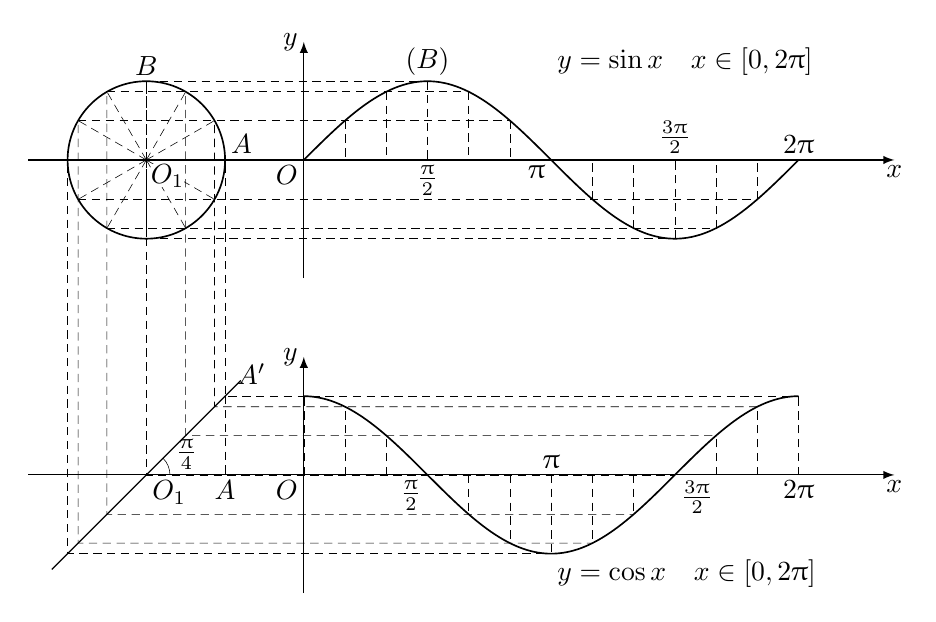
\begin{tikzpicture}[>=latex,scale=1.0,inner sep=2pt]
  \draw[->](-3.5,0)--(7.5,0)node[below]{$x$};
  \draw[->](0,-1.5)--(0,1.5)node[left]{$y$};
  \node at (0,0)[below left]{$O$};
  \draw[->](-3.5,-4)--(7.5,-4)node[below]{$x$};
  \draw[->](0,-5.5)--(0,-2.5)node[left]{$y$};
  \node at (0,-4)[below left]{$O$};
  \draw[semithick,samples=200,domain=0:2*pi]plot(\x,{sin(\x r)});
  \draw[semithick,samples=200,domain=0:2*pi]plot(\x,{cos(\x r)-4});
  \draw[semithick](-2,0)circle(1);
  \foreach \x in {0,1,2,3,4,5,6}
  {
    \draw[very thin,densely dashed](\x/6*pi,{sin(30*\x)})--(\x/6*pi,0);
    \draw[very thin,densely dashed](2*pi-\x/6*pi,{-sin(30*\x)})--(2*pi-\x/6*pi,0);
    \draw[very thin,densely dashed](-2,0)--++(\x*30:1)--({cos(30*\x)-2},{cos(30*\x)-4})--({2*pi-\x/6*pi},{cos(30*\x)-4});
    \draw[very thin,densely dashed](-2,0)--++(-\x*30:1);
    \draw[very thin,densely dashed](\x*pi/6,-4)--++(0,{cos(30*\x)});
    \draw[very thin,densely dashed](2*pi-\x*pi/6,-4)--++(0,{cos(30*\x)});
  }
  \draw(-3.2,-5.2)--(-0.8,-2.8);
  \foreach \x in {0,1,2,3}
  {
    \draw[very thin,densely dashed]({-cos(\x*30)-2},{sin(\x*30)})--({pi-\x/6*pi},{sin(\x*30)});
    \draw[very thin,densely dashed]({-cos(\x*30)-2},{-sin(\x*30)})--({2*pi-\x/6*pi},{-sin(\x*30)});
  }
  \node at (-2,1)[above]{$B$};
  \node at (-2,0)[below right=2pt,inner sep=0pt,fill=white]{$O_1$};
  \node at (-2,-4)[below right]{$O_1$};
  \node at (0.5*pi,1)[above]{$(B)$};
  \node at (0.5*pi,0)[below]{$\frac\uppi2$};
  \node at (0.5*pi,-4)[below left]{$\frac\uppi2$};
  \node at (pi,0)[below left]{$\uppi$};
  \node at (pi,-4)[above]{$\uppi$};
  \node at (1.5*pi,0)[above]{$\frac{3\uppi}{2}$};
  \node at (1.5*pi,-4)[below right]{$\frac{3\uppi}{2}$};
  \node at (2*pi,0)[above]{$2\uppi$};
  \node at (2*pi,-4)[below]{$2\uppi$};
  \node at (-1,0)[above right]{$A$};
  \node at (-1,-3)[above right=3pt]{$A'$};
  \draw[very thin,densely dashed](-1,-3)--(-1,-4)node [below]{$A$};
  \draw[very thin](-1.7,-4)arc(0:45:0.3)node[at start,above right]{$\frac\uppi4$};
  \node at (pi,1)[above right]{$y=\sin x\quad x\in[0,2\uppi]$};
  \node at (pi,-5)[below right]{$y=\cos x\quad x\in[0,2\uppi]$};
\end{tikzpicture}
\end{document}